\documentclass[a4paper,12pt,twoside]{article}
\usepackage[spanish]{babel}
\usepackage[utf8]{inputenc}
\usepackage[T1]{fontenc}
\usepackage{geometry}
\usepackage{graphicx}
\usepackage{float}


\geometry{a4paper, margin=2.5cm}
\title{Aplicaciones en la Ingeniería del Software}
\author{}
\date{}
\usepackage{fancyhdr}
\pagestyle{fancy}
\fancyhf{}
\fancyhead[LO]{Carlos G. Pérez Aranda}
\fancyhead[RE]{Carlos G. Pérez Aranda}
\fancyhead[LE]{Aplicaciones en IS}
\fancyhead[RO]{Aplicaciones en IS}
\fancyfoot[CO,CE]{\textit\thepage}
\begin{document}
\begin{titlepage}
    \centering
    \vspace*{2cm}
    {\Huge \textbf{Aplicaciones en la Ingeniería del Software}}\\[1.5cm]
    {\Large Carlos G. Pérez Aranda}\\[0.5cm]
    {\large \today}\\[2cm]
    \vfill
    
\includegraphics[width=0.8\textwidth]{./images/COLOR_TRANSPARENTE_INFORMATICA.png} 
\end{titlepage}


\newpage
\tableofcontents
\newpage

Existen numerosas aplicaciones de los conceptos discutidos durante el desarrollo de la asignatura Cognición y Comunicación a la ingeniería del software.

Se han abordado diversas áreas del pensamiento, el razonamiento, la creatividad, la dinámica de equipos y los sesgos cognitivos, y explícitamente se 
vinculan muchos de estos conceptos con la práctica de la ingeniería del software.

\section{Pensamiento y Razonamiento:}

\begin{figure}[H]
    \centering
    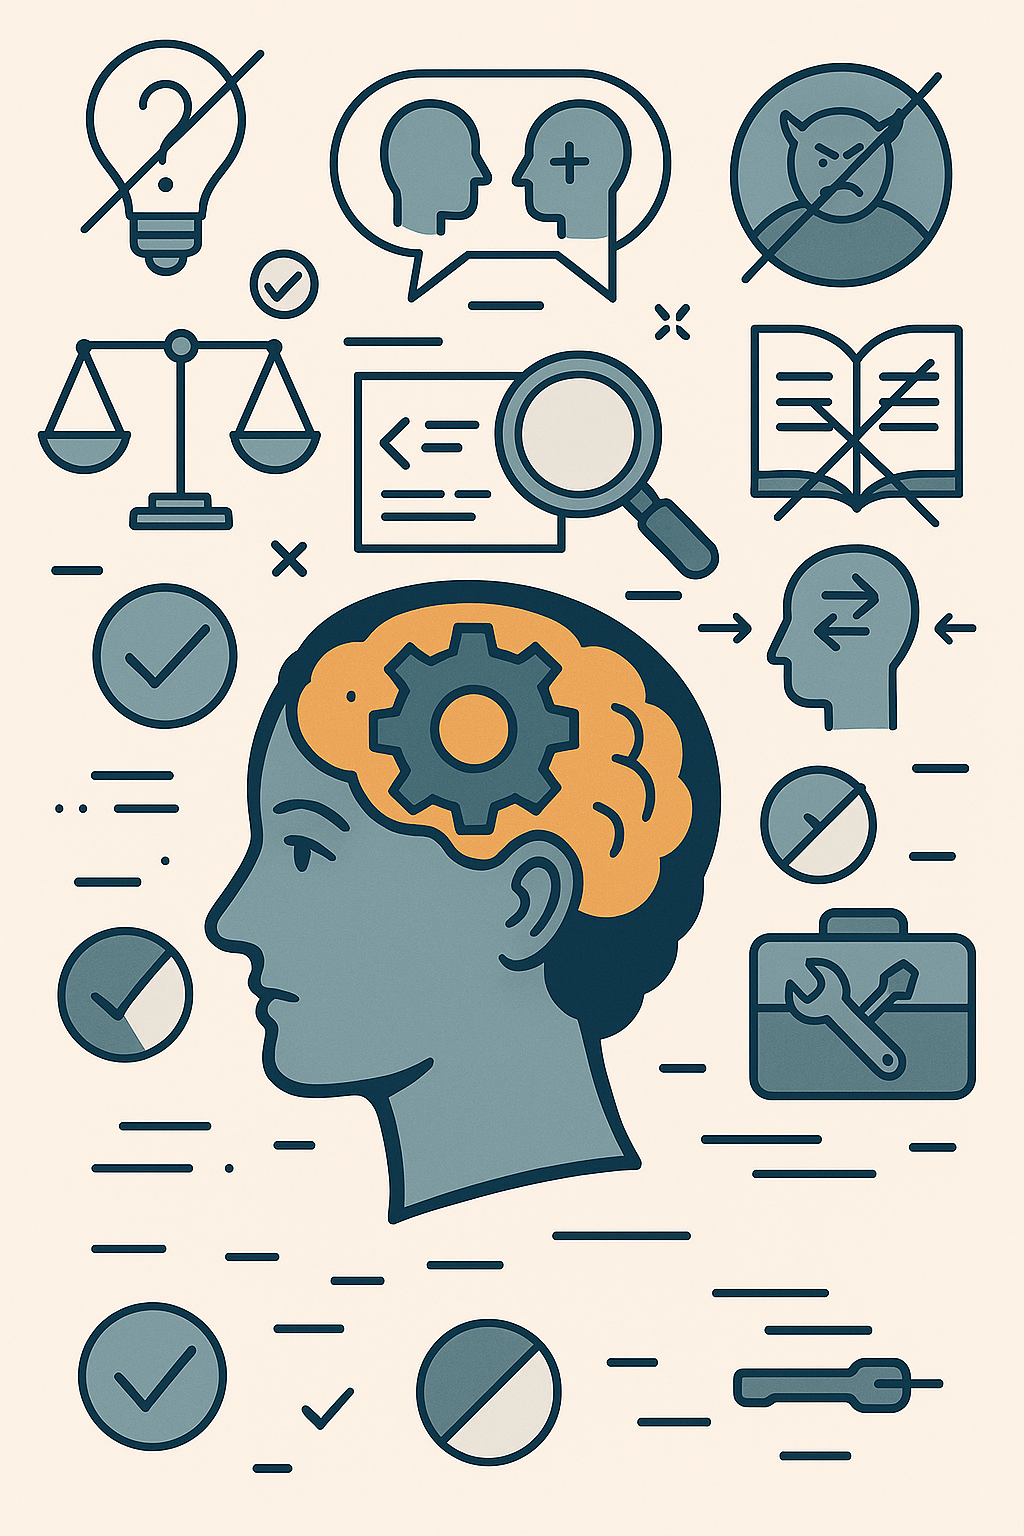
\includegraphics[width=0.6\textwidth]{./images/razonamiento.png}
    \caption{Pensamiento y Razonamiento en Ingeniería del Software}
    \label{fig:pensamiento_razonamiento}
\end{figure}

\begin{itemize}
    \item \textbf{Pensamiento Crítico:} 
    
    El pensamiento crítico es fundamental en la ingeniería del software, permitiendo analizar problemas de manera 
    más objetiva y evaluar situaciones basándose en la razón. Ayuda a tomar decisiones técnicas basadas en hechos verificados y comprobados

    \item\textbf{Cuestionar dogmas o suposiciones establecidas:} 
    
    Asumir una actitud de cuestionar dogmas o suposiciones establecidas es importante, especialmente 
    durante la fase de recopilación de requisitos de un proyecto de software.

    \item\textbf{Identificar y desmantelar falacias lógicas:}
    
    Identificar y desmantelar falacias lógicas mejora la toma de decisiones técnicas al evitar 
    argumentos sin evidencia. También facilita los debates racionales en equipos de desarrollo y 
    ayuda a identificar errores de análisis y causas falsas en bugs o fallos.

    \item\textbf{Comprender los sesgos cognitivos y las heurísticas:} 
    
    Comprender los sesgos cognitivos y las heurísticas es relevante, ya que nuestra mente recurre
    principalmente al Sistema 1 (rápido y automático) en el día a día, lo que puede llevar a errores 
    de juicio donde la precisión es crucial.

    El sesgo de exceso de confianza puede llevar a subestimar tiempos de desarrollo; una solución 
    es usar estimaciones basadas en datos históricos, como el Planning Poker.

    El efecto Google (delegar memoria) implica copiar soluciones sin entender por qué funcionan o 
    qué falló exactamente. Aunque la fuente lo menciona como un problema, la implicación es que 
    se debe contrarrestar adoptando un enfoque más reflexivo.

    Utilizar herramientas objetivas y precisas en lugar de confiar ciegamente en percepciones 
    subjetivas es esencial en ámbitos que requieren precisión. 
    
    Adoptar una actitud crítica y fomentar el hábito de cuestionar es clave donde las decisiones 
    tienen implicaciones relevantes

\end{itemize}

 

\section{Creatividad e Innovación:}
\begin{itemize}
    \item \textbf{Pensamiento Creativo:}
    
    \begin{figure}[H]
        \centering
        
\includegraphics[width=0.6\textwidth]{./images/pensamiento_creativo.png}
        \caption{Pensamiento Creativo en Ingeniería del Software}
        \label{fig:creatividad}
    \end{figure}
    
    El pensamiento creativo es una fuente de innovación en el ámbito empresarial, siendo la capacidad 
    de generar ideas nuevas, de calidad y útiles para resolver problemas. 
    Es complementario al pensamiento analítico.

    Se puede fomentar el pensamiento creativo. En equipos, los procesos de generación de ideas 
    ayudan a superar soluciones convencionales.

    \item \textbf{Técnicas de Creatividad:}
     
    La implementación de técnicas creativas como Design Thinking en fases tempranas del desarrollo 
    de software permite identificar necesidades reales y plantear soluciones creativas, mejorando 
    las expectativas del producto final. Este proceso incluye fases como empatizar, definir, idear, 
    prototipar y evaluar.

    Las reuniones diarias de metodologías ágiles, como Scrum, pueden aprovecharse para generar 
    nuevas ideas y experimentar con ellas.

    \item \textbf{Gestión del Cambio Tecnológico:}

    La gestión del cambio tecnológico y la formación en pensamiento creativo son importantes. 
    Ofrecer planes de formación individualizados potencia la capacidad de innovar.

    \item \textbf{Diversidad en Equipos:}
    La diversidad en los equipos de ingenieros de software (diferentes formaciones, culturas, 
    personalidades) aumenta el potencial creativo. Fomenta el pensamiento creativo y la "lluvia 
    de ideas" (brainstorming), llevando a ideas más variadas y soluciones innovadoras. Fomentar 
    la rotación y mezcla de perfiles es clave para esto.

\end{itemize}

 

\section{Dinámica y Colaboración en Equipos:}

\begin{figure}[H]
    \centering
    
\includegraphics[width=0.6\textwidth]{./images/colaboracion.jpg}
    \caption{Dinamización de Grupos en Ingeniería del Software}
    \label{fig:dinamizacion}
\end{figure}

\begin{itemize}
    \item \textbf{Gestión de Conflictos:} 
    
    La dinamización de grupos se aplica a la gestión de 
    conflictos en ingeniería del software, lo que reduce sesgos y fomenta decisiones colaborativas. 
    La empatía en la gestión de equipos de desarrollo permite mejores relaciones interpersonales y 
    reduce la probabilidad de conflicto. El conflicto es visto como una oportunidad de crecimiento.

    \item \textbf{Comunicación y Colaboración:} 
    
    Una comunicación y colaboración efectiva son 
    cruciales. La conexión entre los miembros del equipo impulsa la productividad y la creatividad.
    Un equipo sólido se basa en la comunicación transparente y la inclusión. Las "soft-skills" son fundamentales para comunicar bien, ir al grano, ser breve y escuchar. Documentar, explicar y colaborar evita "islas de conocimiento".

    \item \textbf{Equipos Positivos:} 
    
    La positividad, entendida como una energía que ayuda a sortear obstáculos y alcanzar objetivos, 
    es fundamental. Los equipos positivos se construyen intencionadamente mediante una cultura de 
    confianza, comunicación y compromiso. Un equipo de software enfrenta obstáculos constantemente, 
    y una actitud positiva y resiliente permite abordarlos sin desmotivación. Recordar la misión 
    diaria es clave para mantener la energía.

    \item \textbf{Reconocimiento y Apoyo:} 
    
    Reconocer los logros, grandes o pequeños, refuerza la 
    moral y el sentido de pertenencia. El apoyo mutuo acelera el crecimiento individual y construye 
    confianza.

    \item \textbf{Retrospectivas Ágiles:} 
    
    Las retrospectivas ágiles potencian la polivalencia y motivación del equipo.

    \item \textbf{Trabajo Remoto:} 
    
    Las técnicas de dinamización de grupos pueden aplicarse al trabajo remoto para reducir 
    malentendidos y fortalecer la colaboración.

\end{itemize}

 

\section{Liderazgo}
    El éxito de un líder no depende únicamente de la inteligencia intelectual o técnica, sino de la 
    inteligencia emocional y social. La inteligencia emocional tiene un mayor impacto en el desempeño 
    del liderazgo y el trabajo en equipo que la inteligencia puramente cognitiva.

    \begin{figure}[H]
        \centering
        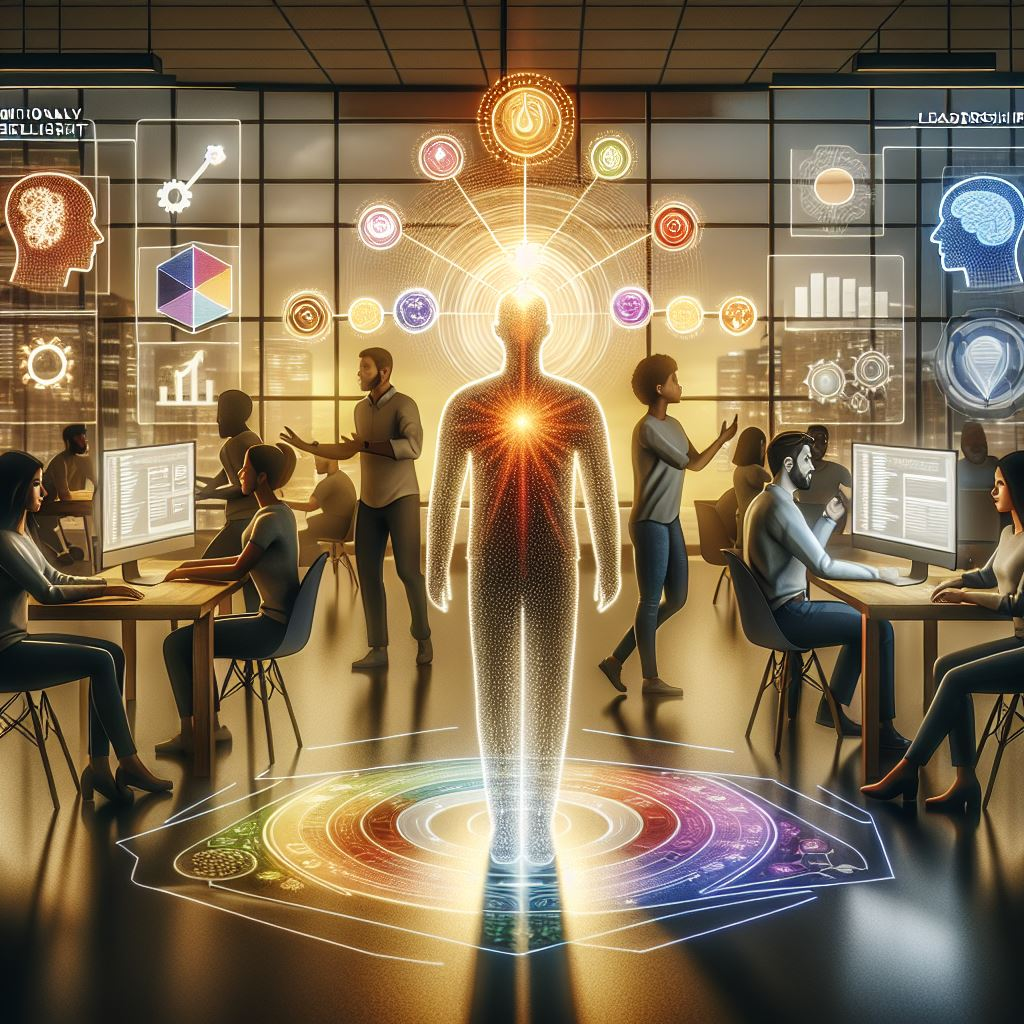
\includegraphics[width=0.6\textwidth]{./images/liderazgo.png}
        \caption{Liderazgo en Ingeniería del Software}
        \label{fig:liderazgo}
    \end{figure}

    \begin{itemize}
        \item \textbf{Inteligencia Emocional:} 
        
        La inteligencia emocional en equipos de desarrollo es fundamental para la comunicación efectiva, 
        gestionar conflictos constructivamente y empatizar durante momentos de presión. Un entorno 
        emocionalmente saludable reduce la rotación, mejora la colaboración y acelera la entrega de 
        software funcional.

        Las competencias de la inteligencia emocional (autoconciencia, autocontrol, motivación, empatía, 
        habilidades sociales) son esenciales para un liderazgo eficaz. Los líderes más eficaces regulan 
        sus emociones, conectan con otros y crean contextos de trabajo emocionalmente saludables.

        \item \textbf{Liderazgo Situacional:}

        La flexibilidad para adaptar los estilos de liderazgo (autoritativo, coach, afiliativo, 
        democrático, marcapauta, coercitivo) según la situación es clave en ingeniería del software. 
        Dominar estos estilos mejora los resultados y el clima laboral.

        \item \textbf{Triple atención del líder:}
        
        La triple atención del líder (hacia uno mismo, hacia los demás, y hacia el sistema) es esencial 
        para un liderazgo técnico maduro.

        \begin{itemize}
            \item \textbf{Atención hacia uno mismo (foco interno):} Previene respuestas impulsivas, 
            favorece la reflexión, el aprendizaje continuo y la estabilidad emocional.
            \item \textbf{Atención hacia los demás (foco en la empatía):} Es crucial para entender y 
            conectar con el equipo.
            \item \textbf{Atención hacia el sistema (foco estratégico):} Permite ver cómo las decisiones 
            afectan al ecosistema (rendimiento, UX, coste, escalabilidad, sostenibilidad) y conectar decisiones técnicas con objetivos de negocio, ayudando a evitar deuda técnica y gestionar el cambio.
        \end{itemize}
    \end{itemize}

    El líder efectivo en software es un conector humano, emocional y estratégico. No solo saber 
    programar bien, sino crear las condiciones emocionales para que otros lo hagan al máximo.

    

\section{Productividad y Hábitos:}

\begin{itemize}
    \item \textbf{Pensar y actuar como profesional:} 
    
    Un manual sobre cómo pensar y actuar como 
    programador profesional es relevante.
    
    \item \textbf{Cartera de conocimientos y experiencia:} 
    
    La cartera de conocimientos y la 
    experiencia son activos profesionales importantes.
    
    \item \textbf{Automatización:} 
    
    Automatizar tareas usando herramientas permite liberar la 
    mente para analizar mejor los problemas.
    
    \item \textbf{Hábitos de código limpio:} 
    
    Escribir código legible, aplicar principios de diseño y 
    detectar ``malos olores'' en el código son esenciales para mantener un código sostenible. 
    Reducen errores, facilitan el mantenimiento y mejoran el trabajo en equipo.

    \begin{figure}[H]
        \centering
        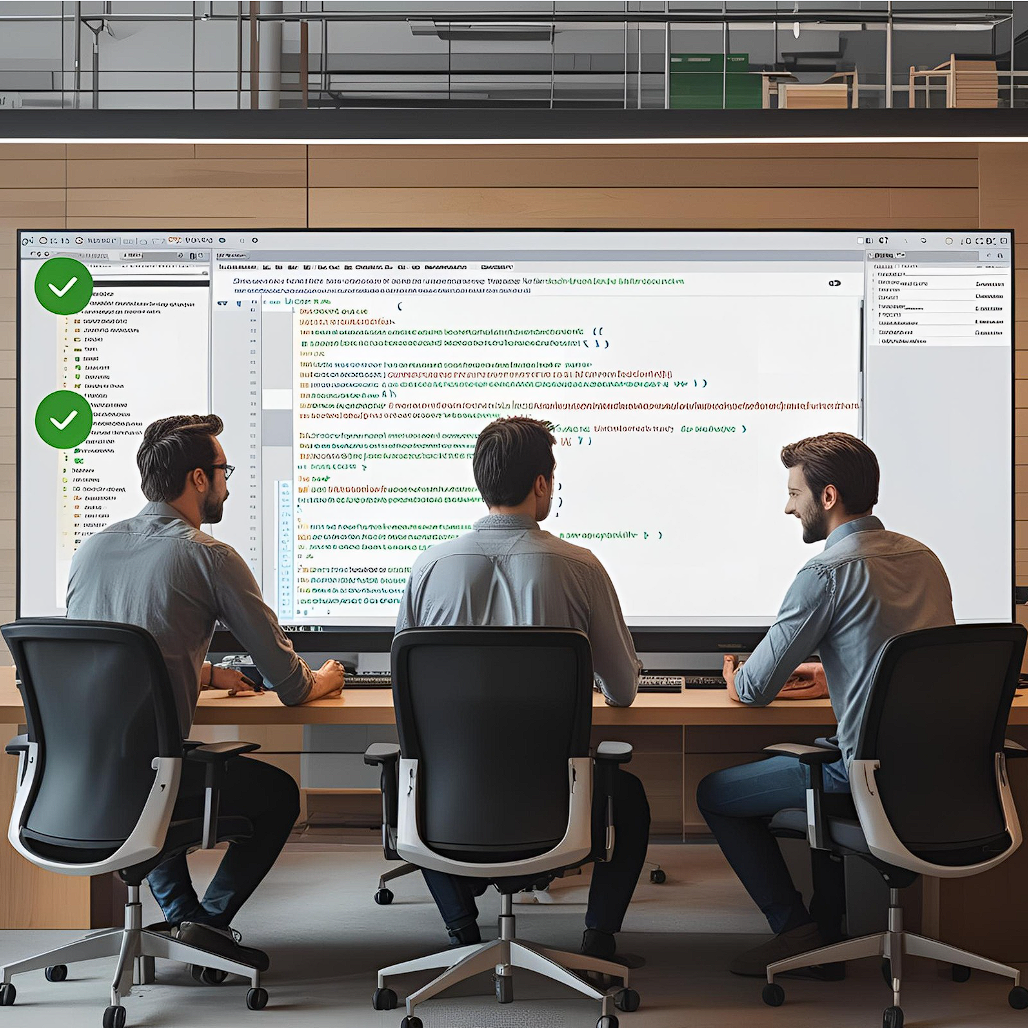
\includegraphics[width=0.6\textwidth]{./images/Productividad.png}
        \caption{Código Limpio en Ingeniería del Software}
        \label{fig:codigo_limpio}
    \end{figure}
    
    \item \textbf{Productividad enfocada:} 
    
    Trabajar en tareas planificadas, terminar lo que se empieza y mantener la productividad 
    ayudan a optimizar recursos y cumplir plazos.
    
    \item \textbf{Aprendizaje continuo:} 
    
    Desarrollar una cultura de aprendizaje continuo es clave para no quedar obsoleto. Aprender 
    algo nuevo cada semana, leer material técnico y trabajar en proyectos personales son hábitos 
    importantes.

    \item \textbf{Adaptabilidad:} 
    
    La adaptabilidad al entorno profesional es importante. Crear un 
    entorno favorable al enfoque en lugares ruidosos o priorizar el valor para el cliente ante 
    decisiones apresuradas son ejemplos.
    
    \item \textbf{Gestión personal del tiempo:} 
    
    Gestionar el tiempo para enfocarse en lo realmente importante y construir rutinas efectivas 
    ayuda a optimizar el uso del tiempo.
\end{itemize}

\section{Comunicación (verbal y no verbal):}

\begin{figure}[H]
    \centering
    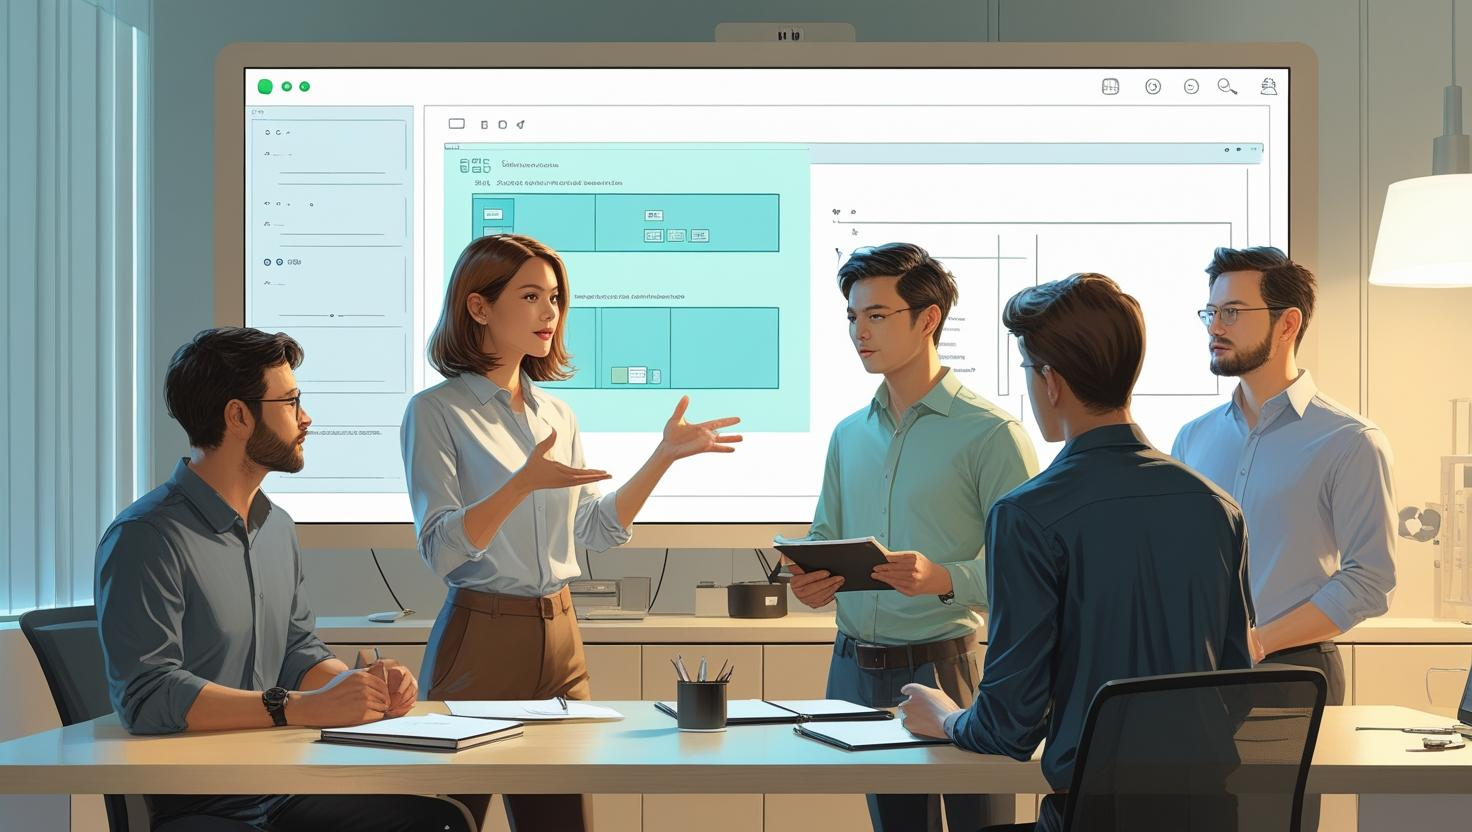
\includegraphics[width=0.8\textwidth]{./images/comunicacion.jpg}
    \caption{Comunicación en Ingeniería del Software}
    \label{fig:comunicacion}
\end{figure}
    \begin{itemize}
        \item\textbf{Soft Skills:} 
        
        Las ``soft skills'' son fundamentales en entornos profesionales reales, donde se trabaja
        en grupo. Comunicar bien es necesario, no solo programar bien. Implica ir al grano, ser breve 
        y escuchar.
        \item\textbf{Islas de conocimiento:} 
        
        No fomentar islas de conocimiento mediante la documentación, explicación y colaboración.

        \item \textbf{Comunicación no verbal:} 
        
        La comprensión y aplicación de la comunicación no verbal son fundamentales.
        \begin{itemize}
            \item En reuniones de equipo, ayuda a detectar si algo no va bien (evadir contacto visual, 
            posturas cerradas, expresiones negativas).
            \item En la presentación de proyectos, permite transmitir confianza (contacto visual, 
            postura abierta, tono de voz seguro).
            \item En la negociación con clientes, ayuda a generar conexión y fluidez (posturas espejo, 
            detectar señales de duda, efecto anclaje).
            \item En entrevistas de trabajo, contribuye a causar una buena primera impresión (actitud, 
            apariencia, efecto halo).
        \end{itemize}
    \end{itemize}

\section{Afrontar errores:}

\begin{figure}[H]
    \centering
    
\includegraphics[width=0.8\textwidth]{./images/depuracion.jpg}
    \caption{Afrontar Errores en Ingeniería del Software}
    \label{fig:afrontar_errores}
\end{figure}

\begin{itemize}
    \item \textbf{En la depuración:} 
    
    El enfoque debe ser arreglar el problema, no buscar culpables. Se debe asumir que el
        propio código es el problema y escribir un test después de corregirlo.

    \item \textbf{Cuadernos de bitácora de ingeniería:} 
    
    Llevar diarios es útil como base de datos de ideas documentadas
        y es más fiable que la memoria.
\end{itemize}

\section{Experiencia de Usuario (UX), Interfaz de Usuario (UI) y Ética:}
\begin{itemize}

    \begin{figure}[H]
        \centering
        
\includegraphics[width=0.8\textwidth]{./images/interfazUX.jpg}
        \caption{UX/UI y Ética en Ingeniería del Software}
        \label{fig:ux_ui}
    \end{figure}
    \item \textbf{Empatía en UX/UI:} 
    
    La empatía es aplicable al Diseño Centrado en el Usuario (UX/UI), poniéndose en el lugar del cliente y usuario para mejorar el diseño.
     También en el Desarrollo de Software Inclusivo.

    \item \textbf{Ética y Responsabilidad:} 
    
    La empatía es relevante para la Ética en la Inteligencia Artificial y Algoritmos y en el Soporte Técnico y Atención al Cliente.

    \item \textbf{Principios de Pre-suasión:} 
    
    Aplicar principios de Pre-suasión (influir antes del mensaje) es útil en UX/UI (dirigir la atención del usuario, motivación), 
    Seguridad (hacer consciente al usuario de peligros), Conversiones (mostrar beneficios) y Gestión de proyectos (crear buen ambiente).

\end{itemize}

\section{Profesionalismo pragmático:}

    Implica asumir la responsabilidad y lidiar con contratiempos profesionalmente.

\begin{itemize}

    \item Evitar la entropía del software (desorden) y la deuda técnica ("no vivir con ventanas rotas").
    \item Ser un catalizador para el cambio.
    \item Recordar el panorama general.
    \item La programación defensiva busca evitar que la aplicación se bloquee, pero a veces es peor un 
    sistema ``tullido'' que uno ``muerto''. 
    Las excepciones no controladas y las herramientas de monitoreo pueden ayudar a detectar problemas.

\end{itemize}


\section{Conclusiones:}
En resumen, en la asignatura y los libros estudiados se nos ha presentado una visión holística de cómo los principios del pensamiento, 
la psicología, la creatividad y la dinámica social son directamente aplicables y cruciales para el éxito en la ingeniería del software, 
mejorando tanto las habilidades técnicas como las interpersonales y el entorno de trabajo.

\end{document}